\documentclass[12pt]{article}

\usepackage{sbc-template}

\usepackage{float}

\usepackage{mathtools}

\usepackage{graphicx,url}

\usepackage[brazil]{babel}
%\usepackage[latin1]{inputenc}
\usepackage[utf8]{inputenc}
% UTF-8 encoding is recommended by ShareLaTex
\usepackage{verbatim}
\usepackage{listings}
\usepackage{xcolor}
\usepackage{fancyref}
\usepackage{hyperref}

\usepackage{fancyhdr}
\fancyhf{}
\cfoot{\thepage}
\pagestyle{fancy}

\definecolor{verde}{rgb}{0,0.5,0}

%para customizar o código (ver https://en.wikibooks.org/wiki/LaTeX/Source_Code_Listings)
\lstset{language=C, %defina a linguagem usada no trabalho
              belowcaptionskip=1\baselineskip,
                breaklines=true,
                frame=false,
                xleftmargin=\parindent,
                showstringspaces=false,
                basicstyle=\footnotesize\ttfamily,
                keywordstyle=\bfseries\color{green!40!black},
                commentstyle=\itshape\color{purple!40!black},
                identifierstyle=\color{blue},
                stringstyle=\color{orange},
                numbers=left,
            }

\sloppy

\title{Otimização do Desempenho na Inversão de Matrizes\\ Universidade Federal do Paraná}

\author{Guilherme Gomes dos Santos\inst{1}}


\address{Bacharelado em Ciência da Computação -- Universidade Federal do Paraná (UFPR)
  \email{ggs12@inf.ufpr.br}
}

\begin{document}

\maketitle

\begin{resumo}
 O trabalho prático da disciplina Introdução à Computação Científica é dividido em duas partes. Na primeira, foi desenvolvido um algoritmo na linguagem C que calculava a inversa de uma matriz, utilizando fatoração LU com pivotamento parcial e refinamento sucessivo. Na segunda parte do trabalho, efetuou-se melhorias no código com o objetivo de melhorar seu desempenho. Este documento apresenta os resultados obtidos após estas otmizações.
\end{resumo}

\section{Introdução}
Durante a primeira etapa do trabalho prático (\textbf{v1}), foi desenvolvido um programa computacional em linguagem C que, dada uma matriz quadrada A de dimensão $n$, devolve a matriz inversa de ${A}$ (${A}^{-1}$), tal que $A {A}^{-1} = I$, onde ${I}$ é a matriz identidade. O algoritmo desenvolvido utiliza eliminação de Gauss com pivotamento parcial, fatoração LU e refinamento sucessivo.

Para a segunda etapa do trabalho (\textbf{v2}), dois trechos do código foram otimizadas de forma a obter uma melhora de desempenho durante a execução do método:
\begin{itemize}
\item Na operação de resolução do sistema linear triangular (\textbf{op1}): $Ly = b; Ux = y$;
\item Na operação de cálculo do resíduo (\textbf{op2}): $R = I - A{A}^{-1}$;
\end{itemize}

Os testes de desempenho foram executados utilizando a ferramenta Likwid, analisando os seguintes aspectos: Tempo médio do cálculo da \textbf{op1} e tempo médio do cálculo da \textbf{op2}, banda de memória (Memory bandwidth [MBytes/s]) do grupo L3, cache miss (data cache miss ratio) do grupo L2 e operações aritméticas (MFLOP/s) do grupo FLOPS\_DP.

A arquitetura do computador utilizado durante os testes de otimização, obtida através da ferramenta likwid-topology, é exibida abaixo:


\begin{table}[H]
\centering
\caption{Processador}
\label{my-label}
\begin{tabular}{ll}
CPU name         & Intel(R) Core(TM) i7-3610QM CPU @ 2.30GHz \\
CPU type         & Intel Core IvyBridge processor            \\
CPU stepping     & 9                                       \\ \hline
Sockets          & 1                                       \\
Cores per socket & 4                                       \\
Threads per core & 2
\end{tabular}
\end{table}

\begin{table}[H]
\centering
\caption{Cache Topology}
\label{my-label}
\begin{tabular}{ll}
Level        & 1                              \\
Size         & 32 kB                          \\
Associativity: & 8                            \\
Cache line size: &  64                        \\\hline
Level        & 2                              \\
Size         & 256 kB                         \\
Associativity: & 8                            \\
Cache line size: &  64                        \\\hline
Level        & 3                              \\
Size         & 6 MB                           \\
Associativity: & 12                           \\
Cache line size: &  64                        \\
\end{tabular}
\end{table}

\section{Estrutura dos dados} \label{sec:firstpage}

Para a primeira etapa do trabalho todas as matrizes foram armazenadas em vetores unidimensionais, visando alocação de memória contígua. Os vetores contendo as matrizes $L$ e $U$ apresentavam as seguintes estruturas:

$L$:

$$ \left(
  \begin{array}{c c c c c}
     1       & 0      & 0      & 0      & 0\\
     l_{10}  & 1      & 0      & 0      & 0\\
     l_{20}  & l_{21} & 1      & 0      & 0\\
     l_{30}  & l_{31} & l_{32} & 1      & 0\\
     l_{40}  & l_{41} & l_{42} & l_{43} & 1 \\
  \end{array} \right)
$$

$U$:

$$ \left(
  \begin{array}{c c c c c}
     u_{00}  & u_{01}    & u_{02} & u_{03}  & u_{04}\\
     0       & u_{11}    & u_{12} & u_{13}  & u_{14}\\
     0       & 0         & u_{22} & u_{23}  & u_{24}\\
     0       & 0         & 0      & u_{33}  & u_{34}\\
     0       & 0         & 0      & 0       & u_{44} \\
  \end{array} \right)
$$

Observa-se que armazenar o conteúdo desta forma é ineficiente, uma vez que todos os zeros das matrizes não são utilizados durante a execução do método.

\section{Otimizações}
\subsection{Estrutura de dados}
O primeiro objetivo durante a \textbf{v2} foi criar estruturas para armazenar estas matrizes de maneira mais eficiente, evitando o desperdício de memória e acesso não contínuo aos dados. As tabelas 3 e 4 demonstram a maneira encontrada para armazenar as matrizes $L$ e $U$.

\begin{table}[H]
\centering
\caption{Matriz L: Vetor melhorado}
\label{my-label}
\begin{tabular}{l|l|l|l|l|l|l|l|l|l|l|}
\cline{2-11}
i   & 0      & 1      & 2      & 3      & 4      & 5      & 6      & 7      & 8      & 9   \\ \cline{2-11}
L[i] & $l_{10}$ & $l_{20}$ & $l_{21}$ & $l_{30}$ & $l_{31}$ & $l_{32}$ & $l_{40}$ & $l_{41}$ & $l_{42}$ & $l_{43}$ \\ \cline{2-11}
\end{tabular}
\end{table}

\begin{table}[H]
\caption{Matriz U: Vetor melhorado}
\label{my-label}
\begin{tabular}{l|l|l|l|l|l|l|l|l|l|l|l|l|l|l|l|}
\cline{2-16}
i   & 0      & 1      & 2      & 3      & 4      & 5      & 6      & 7      & 8      & 9   & 10  & 11  & 12  & 13  & 14 \\ \cline{2-16}
U[i] & $u_{00}$ & $u_{01}$ & $u_{02}$ & $u_{03}$ & $u_{04}$ & $u_{11}$ & $u_{12}$ & $u_{13}$ & $u_{14}$ & $u_{22}$ & $u_{23}$ & $u_{24}$ & $u_{33}$ & $u_{34}$ & $u_{44}$ \\ \cline{2-16}
\end{tabular}
\end{table}

A primeira versão da estrutura de dados, apresentada na\textbf{v1} do código, não é eficiente pois além de armazenar dados desnecessários, gera um acesso não linear aos elementos da matriz: O acesso é organizado em linhas de cache, que são carregadas de uma única vez. Assim, ao acessar o elemento $l_{10}$ por exemplo, os elementos seguintes da mesma linha da matriz L são trazidos dentro da linha de cache. O próximo elemento a ser acessado é o $l_{20}$, que não estará na cache (para um tamanho de linha da matriz suficientemente grande), gerando assim um cache miss.

Assim, ao alinhar os dados nas estruturas descritas os próximos elementos a serem acessados estão sempre na mesma (ou próxima) linha de cache, já que são alocados de maneira contígua. Além disso, consequentemente o tamanho dos vetores é menor: $|L| = (n * (n+1)) / 2 - n$ e $|U| = (n * (n+1)) / 2$ .


\subsection{Código op1}

Para otimizar as estruturas de dados das matrizes $L$ e $U$ foi necessário criar um novo método de percorrer os vetores. Isso ocorre pois cada linha da matriz possui um tamanho diferente, gerando a necessidade de cálculos de índices. Além disso, outra dificuldade surge: o pivotamento parcial executa trocas de linhas nas matrizes $L$ e $U$.

Como a dificuldade para implementar um algoritmo que efetuase estas trocas de linhas em cima dos vetores otimizados seria grande, a decisão foi de manter matrizes auxiliares L\_aux e U\_aux (vetores de dimensão $n * n$) para se efetuar a decomposição LU. Esta alternativa tira proveito do fato de que a eliminação de Gauss com pivotamento parcial é executada apenas uma vez durante o método.

O código abaixo é executado após a conclusão do pivotamento parcial, no qual se efetua uma cópia dos valores úteis contidos nos vetores auxiliares L\_aux e U\_aux para os vetores otimizados L e U.

\begin{lstlisting}
// Inicializa o vetor alinhado L com os valores da matrix inferior
for (i = 0; i < N; i++ ) {
    for (j = 0; j < i; j++) {
        L[index(i,j)] = L_aux[i*N+j];
    }
}

// Inicializa o vetor alinhado U com os valores da matrix superior
for (i = 0; i < N; ++i) {
    for (j = i; j < N; ++j) {
        U[uindex(i,j,N)] = U_aux[i*N+j];
    }
}
\end{lstlisting}

Observa-se que ainda que adicionando esta cópia de dados ao código obtenha-se um ganho em desempenho, e isso é possível por a eliminação de Gauss é executada uma vez, enquanto os vetores L e U serão utilizados número de iterações $* n$ vezes.

Como cada linha dos vetores L e U possui uma dimensão diferente, foi necessário criar as seguintes macros para que a indexação dos vetores fosse feita de maneira simples:

\begin{lstlisting}
#define size(n) (((n)*(n+1))/2)
#define offset(i,j) (size((i)-1)+(j))
#define index(i,j) ((i)<(j) ? 0 :  (offset((i),(j))))
#define uindex(i,j,n) ((i)>(j) ? 0 : (size(n)-size((n)-(i))+(j)-(i)))

//Acessar L[i,j] : L[index(i,j)]
//Acessar U[i,j] : U[uindex(i,j,N)]
\end{lstlisting}

Como visto na disciplina, se um vetor é alocado de forma que seu primeiro elemento não seja mapeado para o primeiro elemento da linha de cache, sempre que esta linha é acessada há dados que são trazidos e não utilizados. Assim, para melhorar a utilização do tamanho da linha de cache (64 Bytes no computador utilizado) os vetores foram alocados com a função posix\_memalign(), garantindo assim que o endereço do espaço de memória alocado seja um múltiplo do parâmetro de alinhamento escolhido.

\begin{lstlisting}
align_L = posix_memalign((void**)&L, 64, lower_size * sizeof(double));
align_U = posix_memalign((void**)&U, 64, upper_size * sizeof(double));
\end{lstlisting}

Percebe\-se então que os vetores L e U são alocados em endereços múltiplos de 64 (tamanho da linha de cache), onde lower\_size e upper\_size são as dimensões dos vetores.

\subsection{Código op2}

Para a otimização da \textbf{op2}, na qual é efetuada a multiplicação das matrizes $A$ e ${A}^{-1}$, o primeiro passo seria otimizar o acesso ao vetor AI contendo a matriz inversa, já que esse acesso é feito por colunas (collumn major order). Como durante a implementação da \textbf{v1} isso já foi levado em consideração, o vetor AI já foi alocado de maneira que o acesso fosse row major order, removendo assim a necessidade de fazer esta otimização na \textbf{v2}.

A seguir é apresentado o código para a \textbf{op2} desenvolvido na \textbf{v1} do trabalho:
\begin{lstlisting}
for (i = 0; i < N; i++) {
	for (j = 0; j < N; j++) {
		soma = 0.0;
		for (k = 0; k < N; k++) {
			soma += A[i*N+k] * AI[k+N*j];
		}
		A_AI[i*N+j] = soma;
	}
}

for (i = 0; i < N; ++i) {
	for (j = 0; j < N; ++j) {
        R[row[i]*N+j] = I[i*N+j] - A_AI[i*N+j];
	}
}
\end{lstlisting}


O foco para otimizar a \textbf{op2} foi manter o código nas especificações necessárias para que o compilador pudesse efetuar e vetorização no loop da operação, possibilitando assim o uso dos registradores AVX. Assim, as estruturas de dados foram alocadas de maneira alinhada:

\begin{lstlisting}
align_A = posix_memalign((void**)&A, 32, N * N * sizeof(double));
align_AI = posix_memalign((void**)&AI, 32, N * N * sizeof(double));
align_R = posix_memalign((void**)&R, 32, N * N * sizeof(double));
\end{lstlisting}

O alinhamento foi feito em 32 bytes para ser compatível com o uso dos registradores AVX, já que cada registrador armazena 256 bits (4 doubles, 8 bytes cada). Além disso, como a vetorização de loops permite a execução de desvios condicionais na forma de atribuição, foi possível remover a utilização da matriz auxiliar A\_AI, economizando assim memória e transferência de dados. O código para a \textbf{v2} ficou:

\begin{lstlisting}
// Primeira versão de otimização
for (i = 0; i < N; i++) {
	for (j = 0; j < N; j++) {
		soma = 0.0;
		for (k = 0; k < N; k++) {
			soma += A[i*N+k] * AI[j*N+k];
		}
		R[i*N+j] = (i == j) ? 1 - soma: 0 - soma;
	}
}
\end{lstlisting}

Outra mudança foi deixar de utilizar o vetor de índices row[i], que era utilizado para armazenar as permutações de linhas efetuadas em R. Essa mudança foi necessária para que não ocorressem acessos fora de ordem no vetor R. Assim o vetor R tem suas linhas trocadas durante o pivotamento parcial para que todos os acessos seguintes aos seus dados sejam em ordem.

A utilização da variável auxiliar \emph{soma} dentro do loop da \textbf{op2} foi necessária para permitir que o compilador GCC gerasse a vetorização. Caso o vetor R fosse utilizado no lugar da variável, o compilador assumiria uma dependência de dados que impossibilitaria a vetorização.

Com estas mudanças e a utilização das flags -fstrict-aliasing e -ffast-math durante a compilação, o GCC conseguiu gerar código vetorizado para utilização dos registradores AVX, isto foi confirmado utilizando a flag -ftree-vectorizer-verbose, que exibe informações referentes ao processo de vetorização. O compilador vetorizou diversos loops do código, e em cada vetorização o cálculo do unroll e \emph{remainder} foi feito automaticamente. Além de vetorizar o loop apresentado na linha 60 do trecho de código acima, ele acabou vetorizando também os loops da \textbf{op1}, que efetuam forward\_substitution() e backward\_substitution().

Ressalta-se a mudança na definição dessas funções, que na \textbf{v2} tornaram-se inline, gerando assim melhora de performance evitando chamadas de funções dentro do loop que é executado $n$ vezes a cada iteração do refinamento.

\subsection{Tentativa de loop unroll na op2}

Buscando melhorar ainda mais o desempenho da \textbf{op2}, foi desenvolvido o seguinte loop unroll exibido no código a seguir.

Com o unroll do laço $j$, o acesso à matriz A é reaproveitado dentro do laço $k$. Assim, a cada iteração em $j$ é calculado os valores de R[i,j], R[i,j+1], R[i,j+2] e R[i,j+3], aproveitando o valor de A[i*N+k] que já está em cache. Assim, o acesso à matriz A, que antes acontecia $N^2$ vezes, é reduzido para $N^2/4$.

De fato esta operação trouxe uma redução no número de caches misses: para $n$ = 2000, o cache miss ratio era em média $0.3364$, reduzindo para $0.2185$ após o unroll. Porém ao comparar resultados da otimização com e sem o loop unroll, constatou-se que embora o unroll proporcionasse a redução de cache miss, a utilização da banda de memória diminuiu drasticamente. Além disso, o tempo de execução médio da \textbf{op2} permaneceu igual ao da \textbf{v1}, ou seja, nenhuma melhoria prática no desempenho.
\begin{lstlisting}
//Segunda versao de otimizacao: tentativa de unroll
for (i = 0; i < N; i++) {           //laco i
	for (j = 0; j < size; ++j) {    //laco j
		soma_v[0] = 0.0;
		soma_v[1] = 0.0;
		soma_v[2] = 0.0;
		soma_v[3] = 0.0;
		for (k = 0; k < N; k++) {   //laco k
			soma_v[0] += A[i*N+k] * AI[j*N+k];
			soma_v[1] += A[i*N+k] * AI[(j+1)*N+k];
			soma_v[2] += A[i*N+k] * AI[(j+2)*N+k];
			soma_v[3] += A[i*N+k] * AI[(j+3)*N+k];
		}
		R[i*N+j] = (i == j) ? 1 - soma_v[0]: 0 - soma_v[0];
		R[i*N+j+1] = (i == j+1) ? 1 - soma_v[1]: 0 - soma_v[1];
		R[i*N+j+2] = (i == j+2) ? 1 - soma_v[2]: 0 - soma_v[2];
		R[i*N+j+3] = (i == j+3) ? 1 - soma_v[3]: 0 - soma_v[3];
	}
}
//Remainder
for (i = 0; i < N; i++) {
	for (j = size; j < N; j++) {
		soma = 0.0;
		for (k = 0; k < N; k++) {
			soma += A[i*N+k] * AI[j*N+k];
		}
		R[i*N+j] = (i == j) ? 1 - soma: 0 - soma;
	}
}
\end{lstlisting}
\emph{Por isso esta tentativa na utilização do loop unroll foi descartada}. Após exaustivos testes, chegou-se a conclusão de que a primeira versão da otimização é melhor: Mesmo com o aumento de cache miss, o tempo médio de execução da \textbf{op1} cai pela metade, a utilização da banda de memória quase dobra.


\section{Resultados}
\subsection{Teste de tempo}

\begin{figure}[H]
\centering
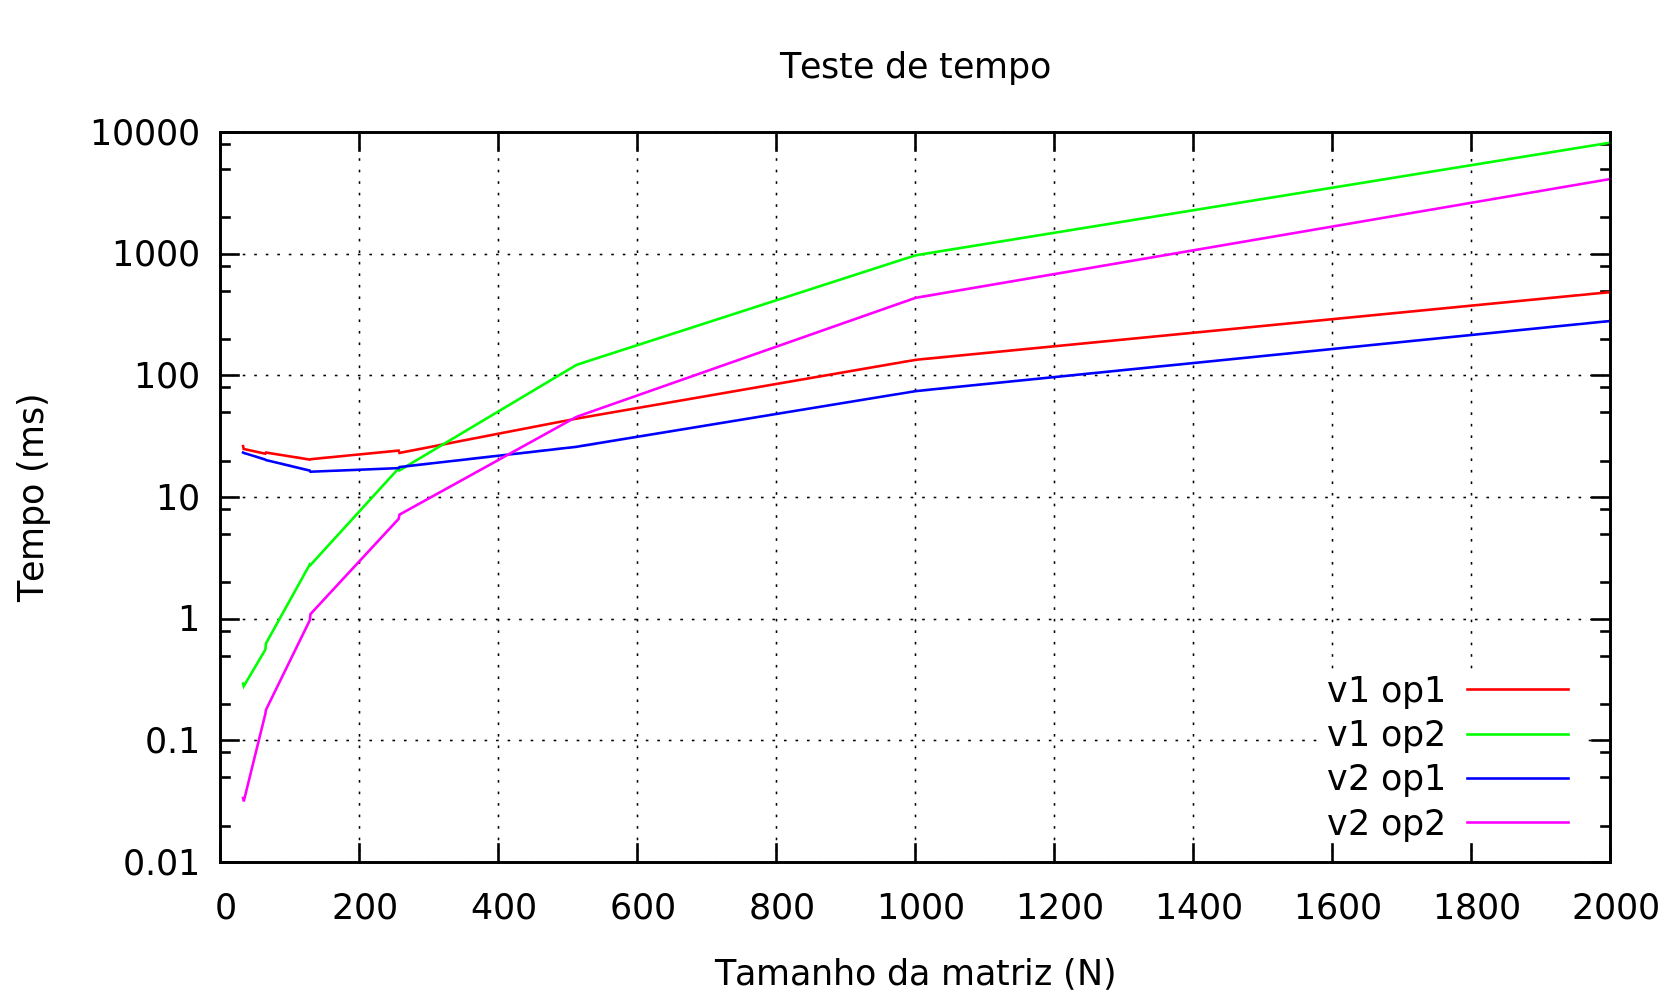
\includegraphics[width=1\textwidth]{img/time.png}
\caption{Tempo médio de execução op1 e op2}
\end{figure}

O gráfico acima apresenta as médias de tempo (em ms) para execução das operações \textbf{op1} e \textbf{op2} em ambas as versões do código. Percebe-se uma grande redução na média de tempo após $n = 256$. Essa redução ocorre principalmente pela utilização de instruções SIMD. Como os registradores AVX passaram a ser utilizados na \textbf{v2}, é esperado que o tempo necessário para executar as operações seja reduzido, uma vez que com AVX as operações são efetuadas em 4 doubles a cada instrução (SIMD). A diferença nos resultados é bastante aparente para matrizes com $n = 2000$ por exemplo, onde a média de tempo na \textbf{v1 op2} era de 8285.02ms e foi reduzida para 4165.51ms na \textbf{v2 op2}.

\subsection{Operações Ariméticas}

\begin{figure}[H]
\centering
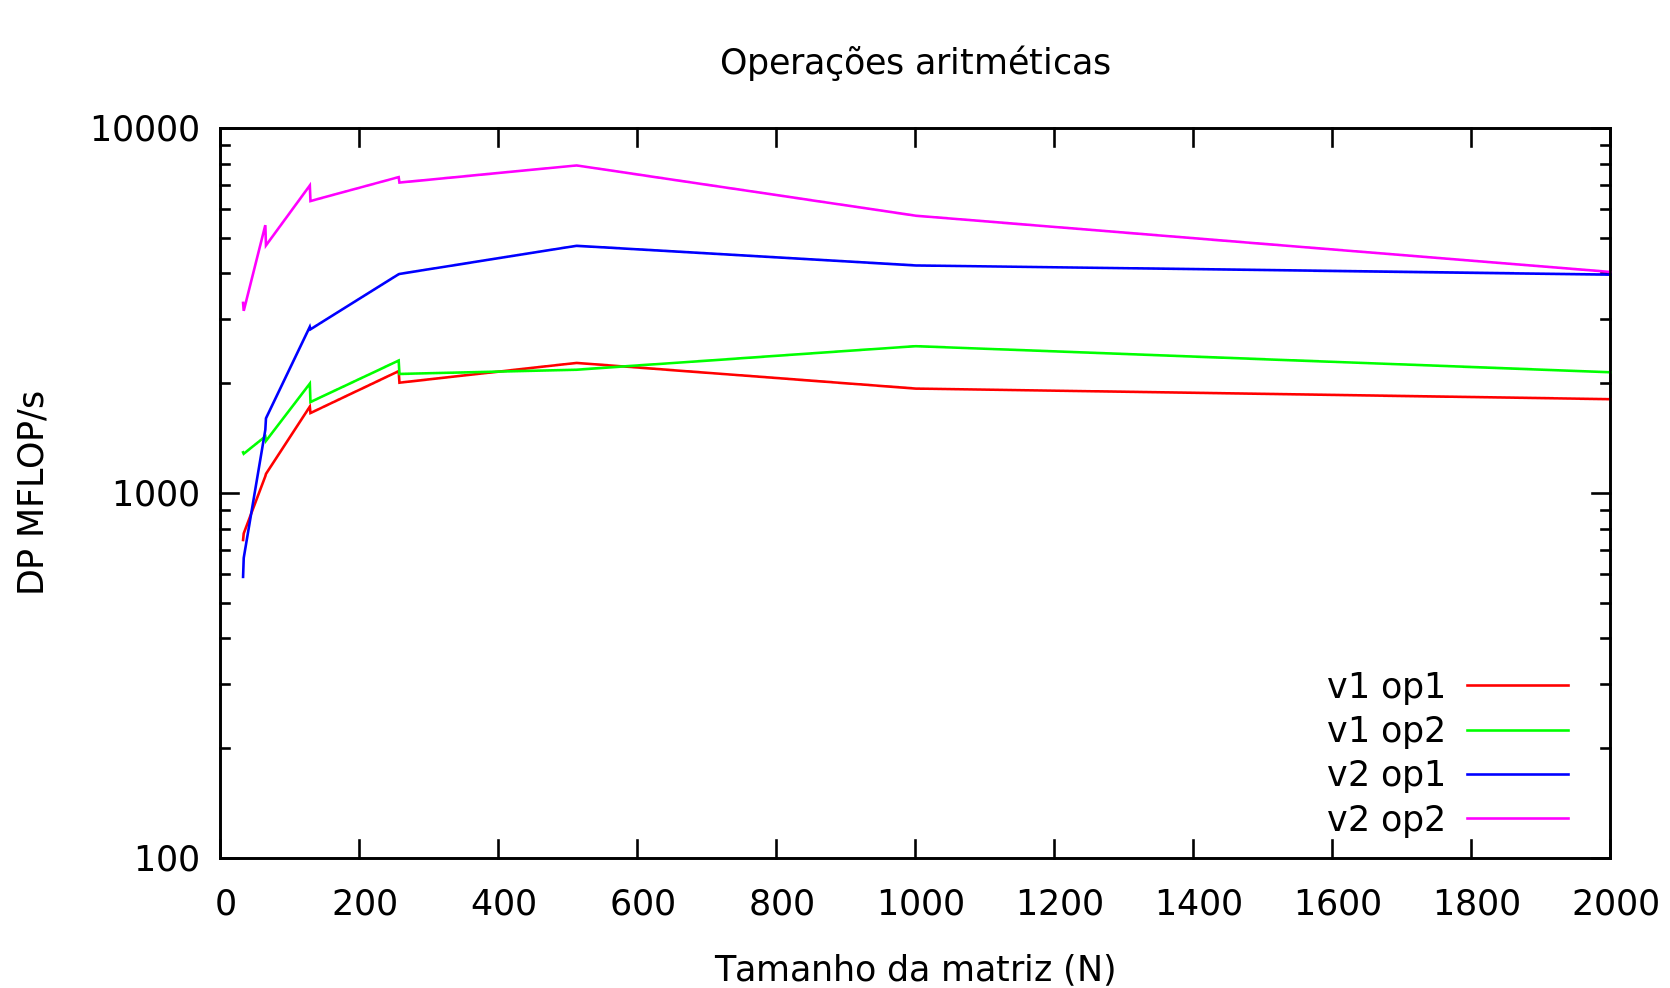
\includegraphics[width=1\textwidth]{img/flops-scalar.png}
\caption{Operações em ponto flutuante}
\end{figure}

As alterações feitas no código somadas às flags corretas possibilitaram ao compilador vetorizar os principais loops contidos nas operações \textbf{op1} e \textbf{op2}. Ao executar o likwid-perfctr monitorando grupo FLOPS\_DP, observou-se que aproximadamente 90\% das operações em ponto flutuante são executadas com AVX. Por consequência, há um grande aumento na quantidade de MFLOPS/s.

Destacam-se as métricas para $n = 512$, em que para a\textbf{v2 op2} as operações em ponto flutuante aumentaram de $2185$ MFLOPS/s para  $7927$ MFLOPS/s, das quais $7844$ são AVX DP MFLOP/s.


\subsection{Banda de memória - L3}

\begin{figure}[H]
\centering
    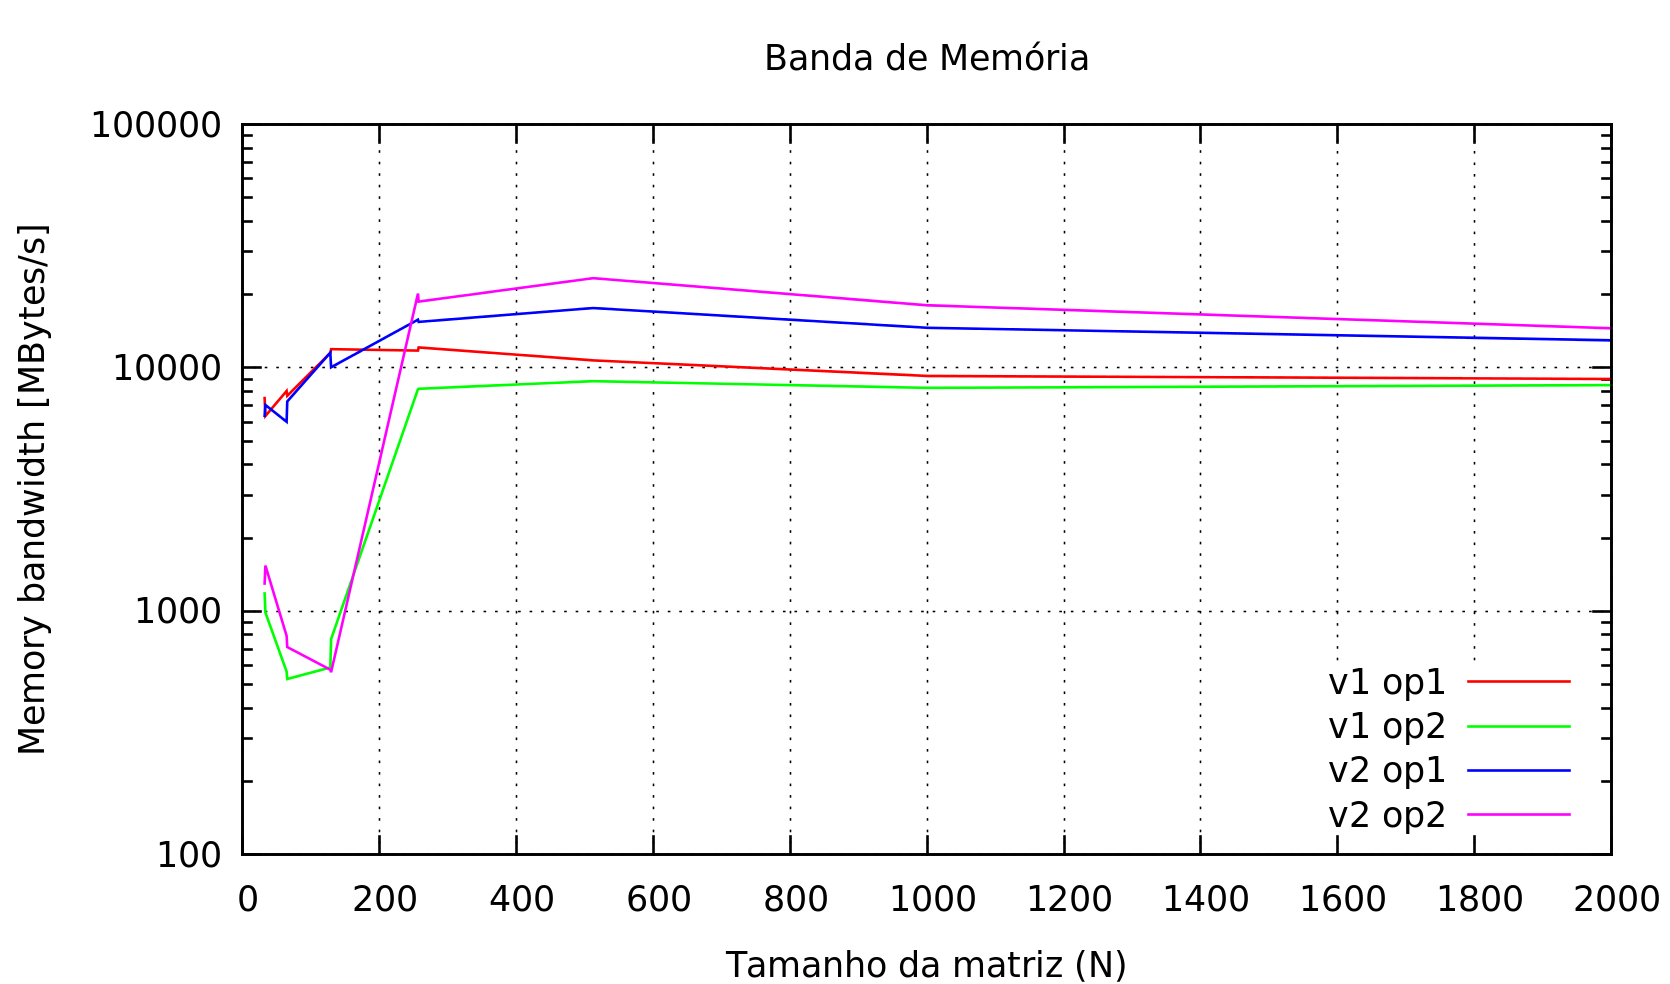
\includegraphics[width=1\textwidth]{img/banda.png}
    \caption{Memory bandwidth na cache L3}
\end{figure}

Como o problema da inversão de matriz é Memory bound, a taxa de transferência de dados entre memória e processador tem um papel fundamental no desempenho geral do algoritmo. As mudanças feitas principalmente na \textbf{op1} possibilitaram um alinhamento de dados mais eficiente. Isso somado à utilização dos registradores AVX gerou um aumento de Memory bandwidth (MBytes/s) para matrizes com $n > 256$.

É possível perceber no gráfico que para matrizes com $n < 256$, a taxa de transferência de dados é baixa. Isso ocorre pois com matrizes dessa dimensão grande parte dos dados cabe na cache L2, reduzindo o acesso à cache L3.

Destaca-se as métricas para $n = 512$, em que a banda para \textbf{op2} era de $8826$ Mbytes/s na \textbf{v1} e passou para $23392$ Mbytes/s na \textbf{v2}.


\subsection{Cache Miss L2}

\begin{figure}[H]
\centering
    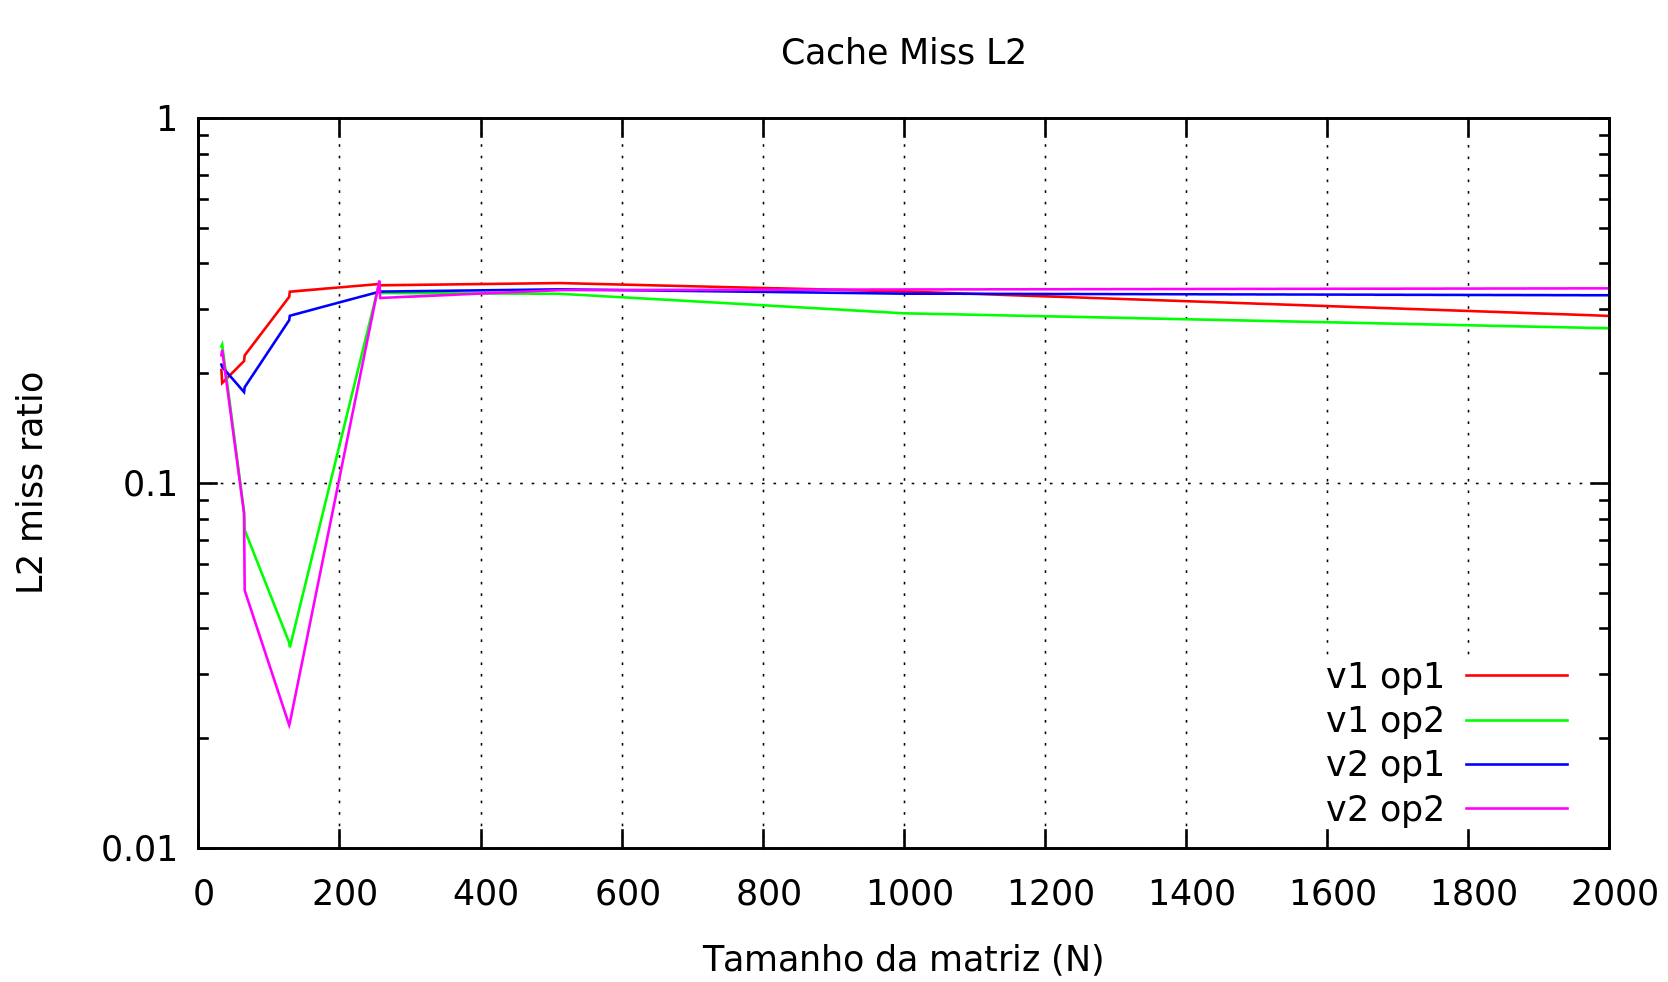
\includegraphics[width=1\textwidth]{img/cachemiss.png}
    \caption{Cache miss - L2}
\end{figure}

O gráfico mostra que não houve redução no número de cache miss (cache miss ratio) na L2. Com as otimizações feitas nas estruturas de dados da \textbf{op1} esperava-se uma redução nestes números, uma vez que na \textbf{v2} os dados estão totalmente alinhados em memória.

Como não houve mudança explicíta de acesso aos dados na \textbf{v2 op2}, é notável que não exista uma redução no número de cache miss. Porém é possível observar que para $n$ a partir de  $1000$ o cache miss na \textbf{v2} tem um leve aumento. Isto pode ter ocorrido devido ao fato do compilador executar as instruções SIMD em uma quantidade múltipla de $4$ de elementos, e executar as operações para os elementos restantes em um laço separado (remainder). O acesso à esses dados restantes ocorre fora de ordem, o que pode aumentar o número da taxa de cache miss.

Observa-se também que como citado anteriormente, para $n < 256 $ a cache miss ratio é muito pequena, ressaltando que para matrizes dessa dimensão os dados permanecem na cache L2, tendo por consequência menos cache miss e uma menor transferência de dados (como visto no gráfico de banda de memória).

\section{Conclusão}

Conclui-se que com um pouco mais de atenção durante o desenvolvimento de um método é possível obter grandes melhoras de desempenho da aplicação. Durante o desenvolvimento do trabalho foi possível experimentar na prática quais conhecimentos são necessários para uma melhor concepção de como melhorar o desempenho do código.

Fazer vários testes com códigos diferentes e comparar quais métricas melhoravam e quais pioravam em cada experimento foi o aspecto mais importante do desenvolvimento, pois percebe-se que não existe uma solução única que irá resolver todos os problemas de desempenho, cabendo ao desenvolvedor possuir o discernimento e conhecimento necessário para avaliar aquilo que trará o maior custo/benefício na performance. Foi interessante perceber que um código utilizando técnicas mais elaboradas não tinha vantagem prática sobre um código relativamente mais simples.

Conseguir reduzir o tempo médio de execução de uma operação pela metade, apenas alocando dados da maneira correta e tirando proveito das ferramentas disponibilizadas pelo compilador foi gratificante.

\section{Referências}

Além do material de apoio da disciplina, estas foram as principais referências utilizadas no trabalho:

\begin{itemize}
\item  Using AVX Without Writing AVX Code -
\url{https://software.intel.com/en-us/articles/using-avx-without-writing-avx-code}
\item Auto-vectorization in GCC - \url{https://www.gnu.org/software/gcc/projects/tree-ssa/vectorization.html}
\end{itemize}


\end{document}
